% Template for PLoS
% Version 3.1 February 2015
%
% To compile to pdf, run:
% latex plos.template
% bibtex plos.template
% latex plos.template
% latex plos.template
% dvipdf plos.template
%
% % % % % % % % % % % % % % % % % % % % % %
%
% -- IMPORTANT NOTE
%
% This template contains comments intended 
% to minimize problems and delays during our production 
% process. Please follow the template instructions
% whenever possible.
%
% % % % % % % % % % % % % % % % % % % % % % % 
%
% Once your paper is accepted for publication, 
% PLEASE REMOVE ALL TRACKED CHANGES in this file and leave only
% the final text of your manuscript.
%
% There are no restrictions on package use within the LaTeX files except that 
% no packages listed in the template may be deleted.
%
% Please do not include colors or graphics in the text.
%
% Please do not create a heading level below \subsection. For 3rd level headings, use \paragraph{}.
%
% % % % % % % % % % % % % % % % % % % % % % %
%
% -- FIGURES AND TABLES
%
% Please include tables/figure captions directly after the paragraph where they are first cited in the text.
%
% DO NOT INCLUDE GRAPHICS IN YOUR MANUSCRIPT
% - Figures should be uploaded separately from your manuscript file. 
% - Figures generated using LaTeX should be extracted and removed from the PDF before submission. 
% - Figures containing multiple panels/subfigures must be combined into one image file before submission.
% For figure citations, please use "Fig." instead of "Figure".
% See http://www.plosone.org/static/figureGuidelines for PLOS figure guidelines.
%
% Tables should be cell-based and may not contain:
% - tabs/spacing/line breaks within cells to alter layout or alignment
% - vertically-merged cells (no tabular environments within tabular environments, do not use \multirow)
% - colors, shading, or graphic objects
% See http://www.plosone.org/static/figureGuidelines#tables for table guidelines.
%
% For tables that exceed the width of the text column, use the adjustwidth environment as illustrated in the example table in text below.
%
% % % % % % % % % % % % % % % % % % % % % % % %
%
% -- EQUATIONS, MATH SYMBOLS, SUBSCRIPTS, AND SUPERSCRIPTS
%
% IMPORTANT
% Below are a few tips to help format your equations and other special characters according to our specifications. For more tips to help reduce the possibility of formatting errors during conversion, please see our LaTeX guidelines at http://www.plosone.org/static/latexGuidelines
%
% Please be sure to include all portions of an equation in the math environment.
%
% Do not include text that is not math in the math environment. For example, CO2 will be CO\textsubscript{2}.
%
% Please add line breaks to long display equations when possible in order to fit size of the column. 
%
% For inline equations, please do not include punctuation (commas, etc) within the math environment unless this is part of the equation.
%
% % % % % % % % % % % % % % % % % % % % % % % % 
%
% Please contact latex@plos.org with any questions.
%
% % % % % % % % % % % % % % % % % % % % % % % %

\documentclass[10pt,letterpaper]{article}
\usepackage[top=0.85in,left=2.75in,footskip=0.75in]{geometry}

% Use adjustwidth environment to exceed column width (see example table in text)
\usepackage{changepage}

% Use Unicode characters when possible
\usepackage[utf8]{inputenc}

% textcomp package and marvosym package for additional characters
\usepackage{textcomp,marvosym}

% fixltx2e package for \textsubscript
\usepackage{fixltx2e}

% amsmath and amssymb packages, useful for mathematical formulas and symbols
\usepackage{amsmath,amssymb}

% cite package, to clean up citations in the main text. Do not remove.
\usepackage{cite}

% Use nameref to cite supporting information files (see Supporting Information section for more info)
\usepackage{nameref,hyperref}

% line numbers
\usepackage[right]{lineno}

% ligatures disabled
\usepackage{microtype}
\DisableLigatures[f]{encoding = *, family = * }

% rotating package for sideways tables
\usepackage{rotating}

\usepackage{verbatim}   % useful for program listings

% Remove comment for double spacing
%\usepackage{setspace} 
%\doublespacing

% Text layout
\raggedright
\setlength{\parindent}{0.5cm}
\textwidth 5.25in 
\textheight 8.75in

% Bold the 'Figure #' in the caption and separate it from the title/caption with a period
% Captions will be left justified
\usepackage[aboveskip=1pt,labelfont=bf,labelsep=period,justification=raggedright,singlelinecheck=off]{caption}

% Use the PLoS provided BiBTeX style
% \bibliographystyle{plos2015}
\bibliographystyle{apalike}

% Remove brackets from numbering in List of References
\makeatletter
\renewcommand{\@biblabel}[1]{\quad#1.}
\makeatother

% Leave date blank
\date{}

% Header and Footer with logo
\usepackage{lastpage,fancyhdr,graphicx}
\usepackage{epstopdf}
\pagestyle{myheadings}
\pagestyle{fancy}
\fancyhf{}
\lhead{
\includegraphics[width=2.0in]{PLOS-submission.eps}}
\rfoot{\thepage/\pageref{LastPage}}
\renewcommand{\footrule}{\hrule height 2pt \vspace{2mm}}
\fancyheadoffset[L]{2.25in}
\fancyfootoffset[L]{2.25in}
\lfoot{\sf PLOS}

%% Include all macros below

\newcommand{\lorem}{{\bf LOREM}}
\newcommand{\ipsum}{{\bf IPSUM}}

%% END MACROS SECTION


\begin{document}

\subsection{Steady-state Approximation of Effective Viscosity}
\label{sec:eff_vic}
We begin with a calculation of a strain rate estimate of the effective viscosity for a network described by our model in the limit of highly rigid filaments.  We carry this out by assuming we have applied a constant stress along a transect of the network.  With moderate stresses, we assume the network reaches a steady state affine creep. In this situation, we would find that the stress in the network exactly balances the sum of the drag-like forces from cross-link slip.  So for any transect of length D, we have a force balance equation.

\begin{equation}
\mathbf{\sigma} = \frac{1}{D}\sum_{filaments}\: \sum_{crosslinks}\xi \cdot (\mathbf{v_i(x)}-\mathbf{v_j(x)})
\end{equation}

where $\mathbf{v_i(x)}-\mathbf{v_j(x)}$ is the difference between the velocity of a filament, $i$, and the velocity of the filament, $j$, to which it is attached at the cross-link location, $\mathbf{x}$. We can convert the sum over cross-links to an integral over the length using the average density of cross-links, $1/l_c$ and invoking the assumption of (linear order) affine strain rate, $\mathbf{v_i(x)}-\mathbf{v_j(x)}=\dot \gamma x$. This results in

\begin{multline}
\mathbf{\sigma} =  \frac{1}{D}\sum_{filaments}\:  \int_0^L \xi \cdot  \: (\mathbf{v_i(s)}-\mathbf{v_j(s)}) \:\frac{ds \cos \theta }{l_c} \\
 = \sum_{filaments}\:  \frac{\xi \dot \gamma L}{l_c} \cos \theta \cdot (x_l + \frac{L}{2} \cos \theta)
\end{multline}

Here we have introduced the variables $x_l$, and $\theta$ to describe the leftmost endpoint and the angular orientation of a given filament respectively.  Next, to perform the sum over all filaments we convert this to an integral over all orientations and endpoints that intersect our line of stress. We assume for simplicity that filament stretch and filament alignment are negligible in this low strain approximation.  Therefore, the max distance for the leftmost endpoint is the length of a filament, L, and the maximum angle as a function of endpoint is $\arccos(x_l/L)$.  The linear density of endpoints is the constant $D/l_cL$ so our integrals can be rewritten as this density over $x_l$ and $\theta$ between our maximum and minimum allowed bounds.

\begin{equation}
\mathbf{\sigma} =  \frac{1}{D} \int_0^L dx_l \int_{-\arccos (\frac{x_l}{L})}^{\arccos (\frac{x_l}{L})}\frac{d\theta}{\pi} \frac{\xi \dot \gamma L}{l_c} \cdot \frac{D}{Ll_c}\cdot (x_l \cos \theta + \frac{L}{2} cos^2\theta)
\end{equation}

Carrying out the integrals and correcting for dangling filament ends leaves us with a relation between stress and strain rate.

\begin{equation}
\mathbf{\sigma} = \frac{(L-2l_c)^2 \xi}{4\pi l_c^2} \dot \gamma 
\end{equation}

We recognize the constant of proportionality between stress and strain rate as a viscosity (in 2 dimensions).  Therefore, our approximation for the effective viscosity, $\eta_{eff}$, at steady state creep in this low strain limit is

\begin{equation}
\label{lin_eqn}
\eta_{c} = \frac{(L-2l_c)^2 \xi}{4\pi l_c^2} .
\end{equation}






\begin{table}[h]
\begin{adjustwidth}{-2.25in}{0in}
\centering
\caption{Simulation Parameter Values}
\label{table:para2}
\begin{tabular}{|c|ccccccc|}
	\hline
	Parameter     & \textbf{Figure 3}          & \textbf{Figure 4}       & \textbf{Figure 5}    & \textbf{Figure 6}  & \textbf{Figure 7}     & \textbf{Figure 8}    & \textbf{Figure 10}          \\ \hline
	$L$           & $1,3,5,7,10$      & $3$             & $5$         & $3,5$       & $5$          & $5$         & $3,5,8$            \\ 
	$l_c$         & $0.2,0.3,0.5,0.8$ & $0.3,0.5$       & $0.3$       & $0.15,0.2,0.3,0.4$ & $0.2,0.3$    & $0.4$       & $0.15,0.2,0.3,0.4$ \\ 
	$\mu_e/\mu_c$ & $100$             & $100$           & $3-300$     & $100$     & $100$        & $100$       & $100$              \\ 
	$\mu_c$       & $0.01$            & $0.01$          & $0.01-0.3$  & $0.001-0.03$    & $0.01$       & $0.01$      & $0.01$             \\ 
	$\xi$         & $0.1,1$          & $0.05,0.1,1$      & $0.01,0.1,1$  & $0.1,1$  & $0.1,1,3.3$ & $0.1,1$    & $0.1,1$           \\ 
	$\upsilon$    & ~                 & ~               & $0.1,0.3,1$ & $0.1,1$   & $0.1,1,3$    & $0.1,1$     & $0.1$              \\ 
	$\phi$        & ~                 & ~               & $0.25$      & $0.5$     & $0.25,0.75$  & $0.25$      & $0.25$             \\ 
	$\tau_r$      & ~                 & $0.1-10^4$      & ~           & ~         & $0.01-10^3$  & $0.01-10^3$ & $10$               \\ 
	$\sigma$      & $0.0002-0.01$     & $0.00003-0.005$ & ~           & ~         & ~            & ~           & ~                  \\
	\hline
\end{tabular}
\end{adjustwidth}
\end{table}


\begin{figure}[h!]
\centering
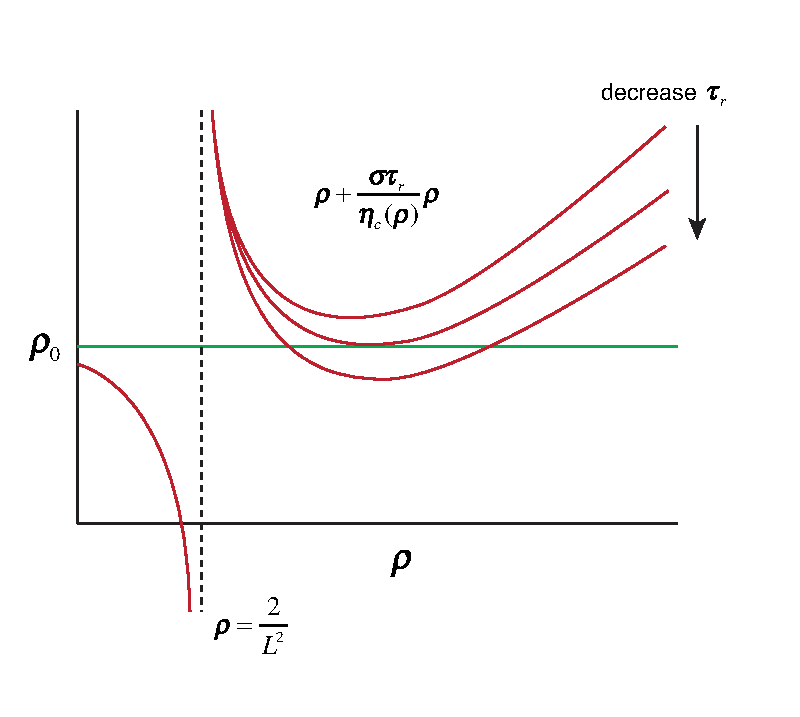
\includegraphics[width=\hsize]{figures/figureS1}
\caption{\label{fig:passive_supp}  Mechanical properties of passive networks.  \textbf{a)} Measurement of elastic phase of deformation in passive networks.  The buildup of strain is approximately exponential and collapse on the predicted strain.  \textbf{b)}  Measurements of elastic modulus of networks (including those in panel a).  Our measurements closely match prediction of $G_0\sim \mu/l_c$.}
\end{figure}

\begin{figure}[h!]
\centering
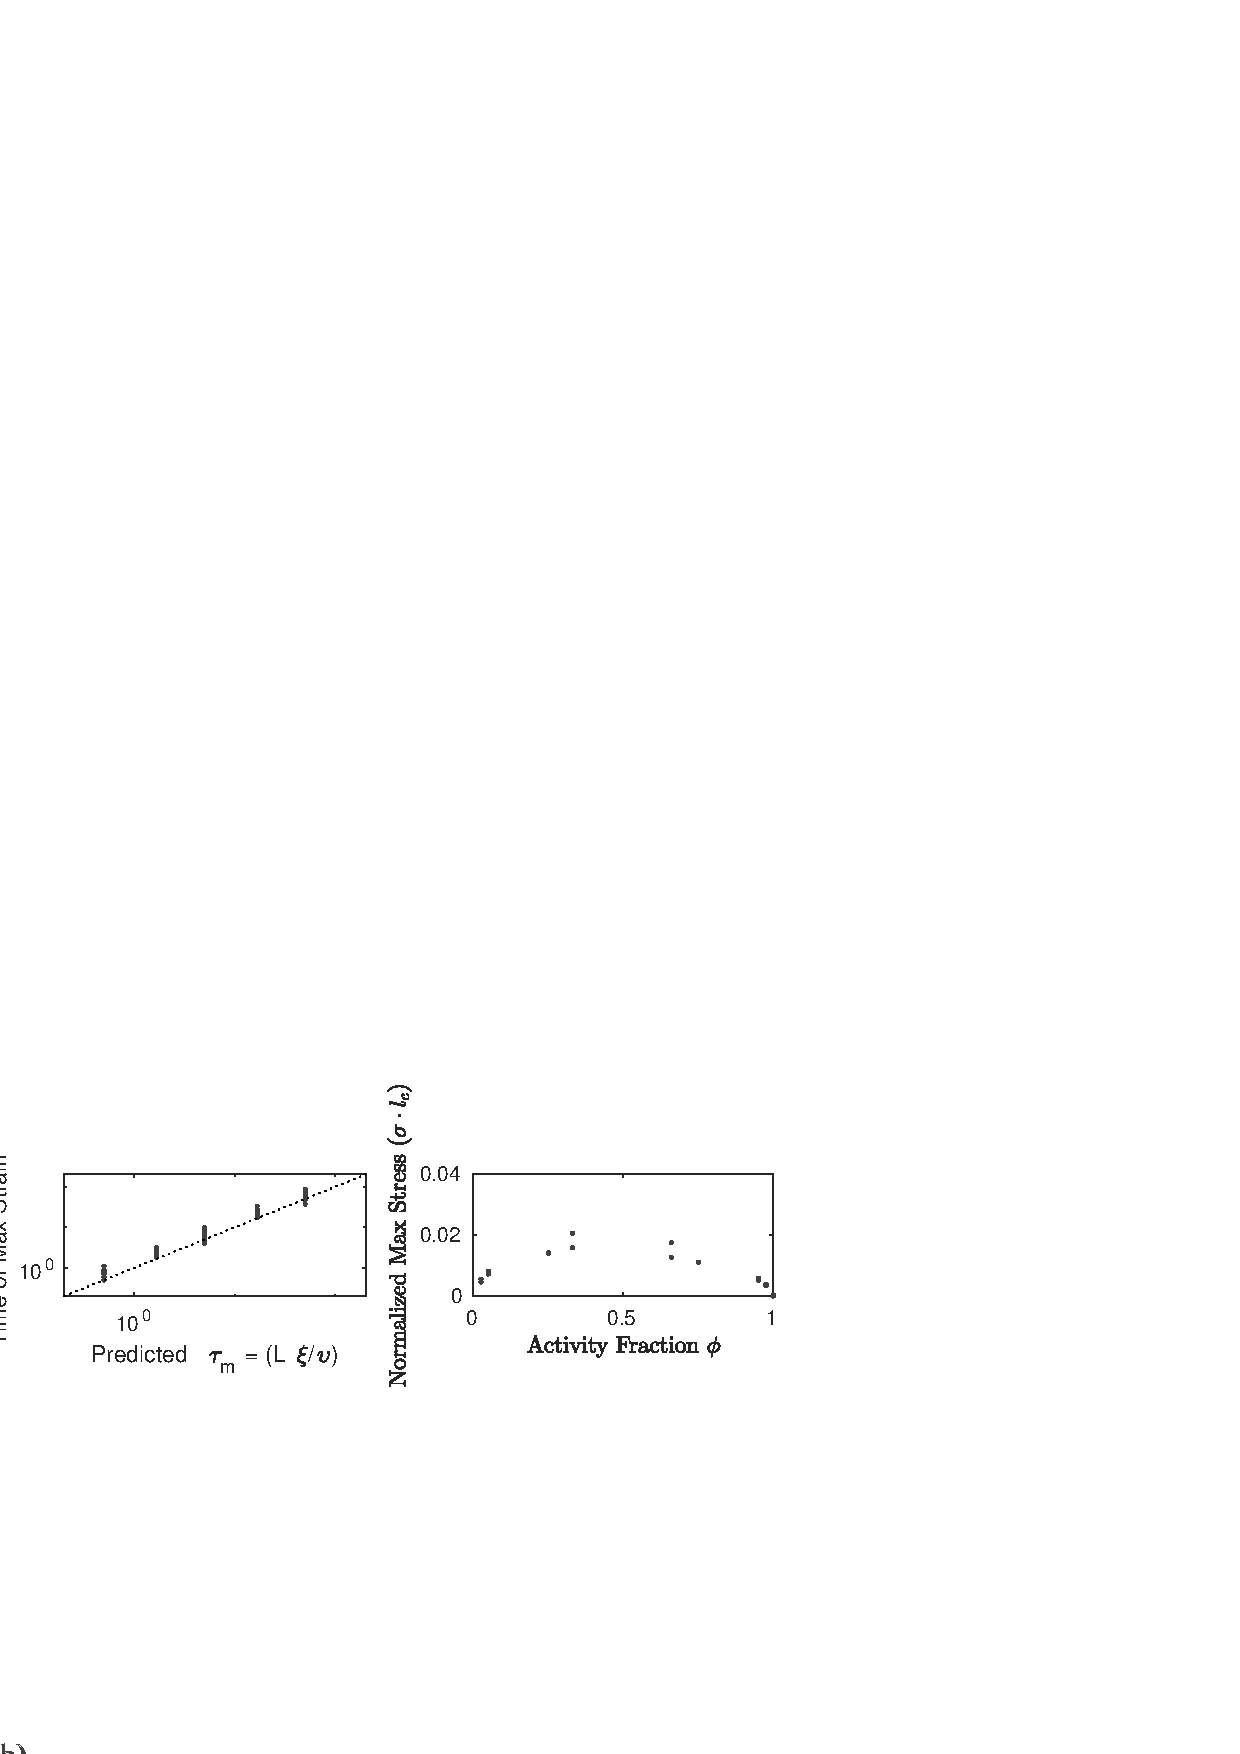
\includegraphics[width=\hsize]{figures/figureS2}
\caption{\label{fig:active_supp}  Mechanical properties of active networks.  \textbf{a)}  Timescale of maximum strain in networks free to contract.  This relationship was found phenomenologically.  \textbf{b)}  Dependence of network stress on the fraction of cross-links which are active.  Note that the network stress approaches 0 as $\phi$ approaches 0 or 1.  \textbf{HEYHEY} The network's ability to deform relies on the magnitude of asymmetric filament compliance.  Total network strain also increases with the applied myosin force $\upsilon$. Note that the extent of contraction approaches an asymptotic limit as the stiffness asymmetry approaches a ratio of $\sim 100$.}
\end{figure}

\begin{figure}[h!]
\centering
\includegraphics[width=\hsize]{figures/figure5_tear}
\caption{\label{fig:active_supp}  Tearing of active networks is prevented via recycling.  \textbf{a)}  An active network undergoing large scale deformations due to active filament rearrangements.  \textbf{b)}  The same network as in a) but with a shorter filament recycling time.  \textbf{c)}  Time trace of internal stresses for network in panel a.  \textbf{d)}   Time trace of internal stresses for network in panel b.  }
\end{figure}

\begin{figure}[h!]
\centering
\includegraphics[width=\hsize]{figures/figure6S}
\caption{\label{fig:combo_prof}  Stress and strain profiles of networks with contractile and passive domains.  \textbf{a)} Blue line indicates strain velocity profile while orange represents net stress as measured in the main text. \textbf{b)} Same as panel a except for the condition where recycling time is 10 s.  Note the increase in net stress and the corresponding increase in flow rate. }
\end{figure}
\end{document}

